% This file was created with tikzplotlib v0.10.1.
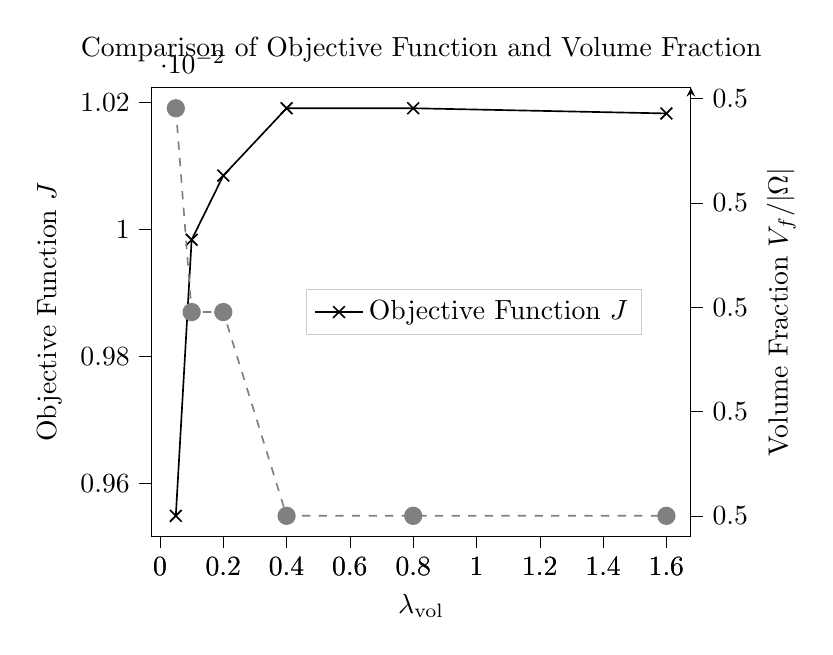
\begin{tikzpicture}

\definecolor{darkgray176}{RGB}{176,176,176}
\definecolor{gray}{RGB}{128,128,128}
\definecolor{lightgray204}{RGB}{204,204,204}

\begin{axis}[
legend cell align={left},
legend style={
  fill opacity=0.8,
  draw opacity=1,
  text opacity=1,
  at={(0.91,0.5)},
  anchor=east,
  draw=lightgray204
},
tick align=outside,
tick pos=left,
title={Comparison of Objective Function and Volume Fraction},
x grid style={darkgray176},
xlabel={\(\displaystyle \lambda_{\mathrm{vol}}\)},
xmin=-0.0275, xmax=1.6775,
xtick style={color=black},
y grid style={darkgray176},
ylabel={Objective Function \(\displaystyle J\)},
ymin=0.00951728223697519, ymax=0.0102223518835069,
ytick style={color=black}
]
\addplot [semithick, black, mark=x, mark size=3, mark options={solid}]
table {%
0.05 0.00954933085727208
0.1 0.00998340694601401
0.2 0.0100843715892529
0.4 0.01019030326321
0.8 0.01019030326321
1.6 0.0101821456334221
};
\addlegendentry{Objective Function $J$}
\end{axis}

\begin{axis}[
axis y line=right,
tick align=outside,
x grid style={darkgray176},
xmin=-0.0275, xmax=1.6775,
xtick pos=left,
xtick style={color=black},
y grid style={darkgray176},
ylabel={Volume Fraction \(\displaystyle V_f/|\Omega|\)},
ymin=0.49990234375, ymax=0.50205078125,
ytick pos=right,
ytick style={color=black},
yticklabel style={anchor=west}
]
\addplot [semithick, gray, dashed, mark=*, mark size=3, mark options={solid}]
table {%
0.05 0.501953125
0.1 0.5009765625
0.2 0.5009765625
0.4 0.5
0.8 0.5
1.6 0.5
};
\end{axis}

\end{tikzpicture}
